\documentclass{acm_proc_article-sp}
\usepackage{graphicx}
\begin{document}
\title{MITM: Logging a Bluetooth Keyboard}
\numberofauthors{2} 
\author{
\alignauthor Kimberly Paterson\\
\affaddr{Cal Poly San Luis Obispo}\\
\email{klpaters@calpoly.edu}\\
\alignauthor Ryan Verdon\\
\affaddr{Cal Poly San Luis Obispo}\\
\email{rverdon@calpoly.edu}\\
}

\date{16 March 2013}
\maketitle

\begin{abstract}
Despite the security improvements made to Bluetooth since its debut in the late 1990s, Bluetooth technology still has many unresolved vulnerabilities that allow for attackers to execute successful Man in the Middle attacks. In particular, the addition of Secure Simple Pairing (SSP) in version 2.1 in 2007 introduced more security flaws, despite it's purpose to secure the pairing process between devices. This work focuses on launching a successful MiTM attack against a Bluetooth-enabled keyboard and a victim PC and logging the data transmitted from the keyboard to the victim PC. Although there is much work done on MiTM attacks and attacking PIN vulnerabilities, there has been little published research on successfully logging the keystrokes from a Bluetooth keyboard using a MiTM attack. 
\end{abstract}


\category{H.4}{Bluetooth Attacks}{Miscellaneous}
%A category including the fourth, optional field follows...
\category{D.2.8}{Software Engineering}{Metrics}[complexity measures, performance measures]
\terms{Theory}

\keywords{MiTM, Bluetooth Attack, Keylogging} % NOT required for Proceedings

\section{Introduction}
Many Bluetooth devices are marketed explicitly for mobile devices such as phones and tablets. 
Attack against tablets not common

threat for MITM attacks is high \cite{sandhya2012analysis}


Many Bluetooth devices are marketed explicitly for mobile devices such as phones and tablets. 
Attack against tablets not common

Public key management is a problem \cite{almonanimitmssp}

\section{Background}
This section discusses the background of Bluetooth and several security features Bluetooth uses.

\subsection{Bluetooth}
Bluetooth is a short-range communications technology used in a wide variety of devices \cite{bluetooth}. The devices Bluetooth are implemented on varies widely from keyboards to fully functional computers \cite{bluetooth}. When two Bluetooth enabled devices are close by each other they can perform what is known as a pairing to connect themselves \cite{bluetooth}. Once the devices are connected they form a piconet and can communicate wirelessly \cite{bluetooth}. Any single Bluetooth device can connect with seven piconets at one time and inside any given piconet there can be up to seven Bluetooth devices connected \cite{bluetooth}. 

\subsection{Bluetooth Security}
Bluetooth implements a variety of security measures to protect itself. Unfortunatly, sometimes Bluetooth ends up defeating its own security measures. The following list are the major security features implemented currently.

\textbf{Frequency hopping}: The Bluetooth protocol cycles through a wide range of frequencies to avoid conflicts and collisons with other Bluetooth devices \cite{ma2007keystroke}. This cycling make it harder to capture packets from a remote host without having special hardware to scan the entire frequency spectrum. Special hardware like the Ubertooth dongle can map out the full spectrum and remotely record packets.

\textbf{Discoverable modes}: Devices that implement the Bluetooth standards can choose to only broadcast their availability for limited durations \cite{ma2007keystroke}. Having a hiden device can prevent against novice attackers from obtaining the Bluetooth address of the hidden device. This can be circumvented by performing a brute force attack on the address space and guessing the hidden devices Bluetooth address \cite{ma2007keystroke}.

\textbf{PIN authentication}: To pair two Bluetooth devices together there are several authentication options. One of the most secure options is when a PIN is used on both devices to confirm who the other person is \cite{ma2007keystroke}. Sadly, there exists a mode where no-PIN is needed that can be defaulted to thereby removing any security protections. Also, even if a PIN is used it is only numeric characters which makes it much easier to crack \cite{ma2007keystroke}.

\textbf{Security Modes}: Bluetooth devices can be in a variety of different security modes with varying levels of security \cite{ma2007keystroke}. For backwards compatability reasons the lowest level of security can still be used.

\begin{enumerate}
\item Mode 1: no security or encryption
\item Mode 2: no security until channel is established on L2CAP level (software)
\item Mode 3: has security before link setup on the LMP level (hardware)
\item Mode 4: introduced Secure Simple Pairing, pairing protocol to protect devices while a pairing is completed
\end{enumerate}

\subsection{Secure Simple Pairing (SSP)}
Secure Simple Pairing (SSP) was introduced in revision 2.1 and has remained largely unchanged in the subsequent versions, although some of the authentication protocols have changed \cite{barnickel2012implementing}. The original purpose of SSP was to simplify the pairing process for the end-user and to improve security, especially against MITM attacks \cite{sandhya2012analysis}. In order to simplify the process, 4 different association modes were created, and are used depending on the capabilities of the devices. The 4 association models are as follows:

\textbf{Numeric Comparison}: a 6 digit number is displayed on both devices and a user confirms that the numbers match (this is designed for devices that both have display and input capabilities)\\\\
\textbf{Passkey Entry}: designed when one device has input (keyboard) and the other mostly display; the device that has the display shows a 6 digit number, which the user types in on the input device.\\\\
\textbf{Just Works}: one device has no input or display; the user must accept the connection without being able to visualize that the numbers are the same (more in nist)\\\\
\textbf{Out of Band (OOB)}: designed to connect when two devices are touched together, (e.g. Near Field Communication or NFC)\\\\
%TODO 5 steps of pairing protocol
\subsection{MITM Bluetooth Attacks}
We focus on man-in-the-middle attacks (MITM) against devices that use Passkey Entry as their primary mode of authentication for pairing. Historically, these attacks have been simple to implement and successful using a variety of approaches.  

Among the vulnerabilities NIST lists for Bluetooth versions before 4.0 is the weakness of one-way-only challenge and response authentication used in SSP \cite{scarfone2008guide}. 
Since Bluetooth devices often do not have display or input capabilities, Passkey Entry or Just Works modes for SSP are necessary to connect less-functional devices, such as keyboards, to more functional devices such as computers or tablets. When only one device is asking for authentication, it's possible to spoof the keyboard into pairing into Just Works mode and impersonate the keyboard to the victim computer. Despite NIST's statement that the one-way-only challenge affects versions before 4.0, if an attacker can force a keyboard into Just Works mode, it becomes vulnerable to MITM attacks.

\subsubsection{Pin Vulnerabilities}
NIST recommends that users use a 6-digit random pin when authenticating either in Numeric Comparison or Passkey Entry mode, however, this feature is not mandated. Some operating systems may allow for fewer than 6-digit pins, which are less secure, or let users enter custom pins, which will not be random. Assuming developers follow the recommended protocol, the probability of guessing the pin is one in a million according to NIST \cite{scarfone2008guide}. 

Additionally, NIST claims that since the 6-digit passkey is not incorporated into the link key generation, it isn't useful for an eavesdropper to use. Nonetheless, Lindell showed in 2008 that the pin becomes useful to an attacker when attempting to pair with a device when the passkey is used more than once \cite{lindell2008attacks}. Knowing the pin can allow an attacker to connect with the device when the victim attempts to connect his/her devices again. It is possible to force a user to re-pair their devices either by DoS \cite{cuthbertbluetooth} or by making the victims assume that the victim devices forgot the link key\cite{shaked2005cracking}. When the devices try to pair again, an attacker can intercept the process and authenticate itself to each device. 

If the attacker does not know the pin, he/she can, in fact, crack it as Shaked and Wool showed in 2005 when they were able to crack a 4-digit pin in 0.27 seconds by observing Bluetooth traffic \cite{shaked2005cracking}. Similarly, in 2012, Barnickel, Wang, and Meyer were able to able to execute a MITM attack by first jamming the connection between the connected devices, calculate the passkey and then re-pairing with the devices \cite{barnickel2012implementing}. Both works and Lindell's work exploit the vulnerabilities of the Passkey Entry protocol, where the bit-by-bit evaluation of the passkey by devices can be used to leak the passkey a bit at a time, to determine the passkey quickly. As these works show, computing the pin is alarmingly simple and fairly useful when pins are reused; currently, this is still a feasible attack, but is less likely when pins are not fixed (such as with headsets or other fixed-pin devices).

\subsubsection{Key Logging}
Regardless of how infeasible it is to guess the password when it is not being reused, some successful approaches target Passkey Entry mode since attackers can force a user to enter the passkey for them. This is especially useful for devices that rely on Passkey Entry such as Bluetooth keyboards, which do not necessarily have display capabilities and use one-way authentication. Typically, Bluetooth enabled keyboards will connect to a device with display capabilities (e.g. a tablet or PC) and the device will display a passkey that the user must input through the connected keyboard. If an attacker can trick the user into entering the passkey for him/her, sidestepping the pin guessing process becomes quite easy. 

The benefit of attacking a keyboard in this way is having direct access to the data being imputed into the keyboard without the need for physical access to the device or the software on either the keyboard or device it's connected to. Additionally, if an attack can successfully execute a MITM attack by logging the keyboard input and then forwarding the data to the victim PC or tablet, the user may not even be aware that their data are compromised. 

Keylogging with a MITM attack is theoretically possible and some work has been done toward a seamless attack of this sort. In 2007, Ma, Mbugua, and Poon were able to use a pin attack against a paired computer and keyboard by sniffing the Bluetooth traffic and cracking the pin \cite{ma2007keystroke}. However, they concluded that keylogging was infeasible because of the cost. A more successful approach was done by Cuthbert et al. where they first performed a DoS attack to disconnect the PC from the keyboard, and then tricked the keyboard into pairing with their attack PC in unencrypted mode \cite{cuthbertbluetooth}. The attack PC then sends a link request to the victim PC, which connects through the first few stages of authentication and then displays a pin for the user to enter. Thinking that this is a malfunction of the connection, the user unwittingly types the passkey to the attack PC, which then enters the pin into the victim PC. Although Cuthbert et al. were able to connect to both devices, they did not execute a successful keylogger, although they argued it would not have taken much more work. 

Our work is based on this last approach, but we implement a successful keylogger that forwards the user's data to the victim device.

\section{Related Work}
MITM attacks are commonly researched for Bluetooth technologies and there are a variety of approaches to executing the attacks. As previously mentioned, the PIN prevents potential issues and is vulnerable to social engineering attacks. Phan and Mingard show that a malicious device can impersonate a legitimate device and communicate with another legitimate device by making the user enter whichever authentication pin it chooses \cite{phan2012analyzing}. Other approaches target reused pins by eavesdropping on the pairing process, jamming the signal, and then attempting to pair to the devices using the already-used pin \cite{barnickel2012implementing}. These approaches rely on the victim not thinking critically about the pin -- in some cases, the pin is hard-coded and so must be reused, or is set to default, or the user will use the same pin out of convenience. For this reason, these attacks rely on user-error, which does contribute largely to MITM exploits.  

Another interesting approach is the BT-Nino-MITM attack or Bluetooth No Input, No Output attack \cite{4401672}
. In this attack, the attacker forces the victim device into \textit{Just Works} mode, which does not provide any encryption or authentication. The attacker then jams the physical layer by hopping frequencies along with the victim and sends fake data. The authors also propose jamming the entire 2.4GHz frequency to for the user to try \textit{Just Works} mode. 

\section{Threat Model}
TODO

\section{Attack Overview}
Based on prior research, the theoretical attack would take 4 main steps to executing the attack, which are as follow:
\begin{enumerate}
\item Find Bluetooth Address of the keyboard
\item Execute DoS attack against victim
\item Pair with keyboard and victim
\item Forward keystrokes to victim
\end{enumerate}

Each step is outlined in detail in the following subsections.

\subsection{Finding the Keyboard Bluetooth Address}
Obtaining a device's Bluetooth address is quite simple. If the device is in discoverable mode, then the address is easily found using a Bluetooth scanner or command line tool such as \texttt{hcitool scan} from the Bluez Linux utilities. If the device is not in discoverable mode, but is connected to another Bluetooth-enabled device, then the address can be found using a Bluetooth sniffer and packet capturing software such as Kismet\cite{kismet}. Project Ubertooth \cite{ubertooth} provides both hardware and a plugin for Kismet that allows you to promiscuously sniff Bluetooth packets and then displays the Bluetooth address from whatever device is sending out the packets. Without pairing to the device, it is possible to sniff the packets from nearby devices, although the data is likely encrypted, and obtain the address \cite{hak5}. 

In order to execute the attack, the attacker will need to know the Bluetooth address for both the keyboard and the victim PC. If the attacker does not have access to hardware like Ubertooth One, he or she can obtain the BT address after performing a DoS attack, at which point the user may make the devices discoverable in order to reconnect the devices and the attacker can scan for the devices. 

\subsection{DoS Attack}
The purpose of the Denial of Service attack (DoS) is to trick the user into initiating pairing. Although devices, once paired, do not technically need to be re-paired, a user who is frustrated with Bluetooth not connecting may try to pair the devices again to re-initiate the connection. Ultimately, this means the devices become discoverable to the attacker, who swiftly swoops in to pair with both devices. 

There are several known approaches to doing a DoS attack against Bluetooth and DoS attacks present a realistic problem for Bluetooth users \cite{bandyopadhyay2010information}; an attacker can force some operating systems to disconnect with a keyboard by spamming the victim PC with link requests \cite{cuthbertbluetooth}. This attack worked for Windows Vista and Linux Ubuntu with BlueZ but did not work for Windows 7; as a result, if the attacker does not know what OS the user has installed, this approach may not be effective. 

Another way to perform DoS is to jams the frequency the device is operating on in order to force the user into re-pairing. The attacker can jam the Bluetooth 2.4GHz frequency or frequency hops with the victim and sends fake data \cite{4401672}. Once the attacker jams the signal, he or she can attempt to connect using a reused pin\cite{barnickel2012implementing}, which is effective against poor random pin generation or user-generated pins that some operating systems implement. 

\subsection{Getting in the Middle}
What makes this attack possible is the unreliability of Bluetooth connections. Users often experience problems connecting devices and understand that disconnections between their devices are common, so service interruptions are not out of the ordinary and are not suspicious. To fix connections, as in the case of a DoS attack, users will often try to re-pair their device or toggle the connect switch or button to try and connect the devices again. Once the user makes his or her devices discoverable, the attacker can quickly pair with both devices. The process must be executed quickly so that the victim keyboard does not have time to connect to the victim PC. 

The first step is to pair with the victim keyboard and connect in unencrypted mode, or security Mode 1. This means all data coming from the keyboard will not be encrypted and can be easily dumped and extracted later. If the attacker is successful in pairing with the keyboard and connecting in unencrypted mode, the keyboard is no longer discoverable, which means it will not show up as "available" on the victim PC's Bluetooth device manager. 

The second step is to change the BlueZ configuration file to mimic the appearance of the user's keyboard. When the keyboard becomes discoverable \texttt{hcitool scan} can give you the name of the device, which the attacker simply change in the Bluetooth config file (found in \texttt{/etc/bluetooth/main.conf} for Ubunutu 12.04). The attacker must also change the device class so that the device will show up as a keyboard in the device manager of the victim PC. Typically this device id is \texttt{0x000540} for keyboards. 

At this point, the attacker relies on the victim thinking the attacker's "keyboard" is his or her own device (since the victim may not see the actual keyboard in the device manager any longer). The victim, thinking the keyboard is familiar, initiates a pair request to the attacker's PC. Typically, the victim PC will now prompt for a pin from the attacker, but since the user thinks the victim PC is connecting to the victim keyboard, the user enters the pin on the Bluetooth keyboard, which is then forwarded from the attacker to the victim PC, completing the pairing process. 

\subsection{Forwarding}
Although the attacker has now positioned him or herself between the keyboard and the victim PC, the attacker must effectively forward the keystrokes coming from the keyboard to the victim PC, otherwise the jig will be up.   
Theoretically, it's possible to capture the Bluetooth packets from the keyboard, alter the source address to be the attacker's PC Bluetooth address and then forward the packets using C. However, we were unable to parse the Bluetooth packets because of the implementation differences in libpcap between Bluetooth and Ethernet traffic. 

We were able to find a work-around considering that our attacker PC is simply emulating a keyboard; therefore, we looked for HID clients that mimic keyboards and use Bluetooth. We found an Linux tool called hidclient \cite{hidclient} which can essentially forward from any input device on the attacker PC. 

Hidclient allows the user to forward from any input device the user specifies and that the computer recognizes as a valid input. Since the victim's Bluetooth keyboard is connected to the attacker already, hidclient recognizes the keyboard as an input source. This means the attacker's keyboard is free for typing and will not appear on the victim's screen. The keystrokes are forwarded on to the victim with minimal delay. 
\begin{table}
\begin{tabular}{|c|c|}
\hline
Key Value & hcidump Encoding\\\hline
A&0x04\\
B&0x05\\
C&0x06\\ 
D&0x07\\
E&0x08\\
F&0x09\\
G&0x0A\\
H&0x0B\\
I&0x0C\\
J&0x0D\\
K&0x0E\\
L&0x0F\\
M&0x10\\
N&0x11\\
O&0x12\\
P&0x13\\
Q&0x14\\
R&0x15\\
S&0x16\\
T&0x17\\
U&0x18\\
V&0x19\\
W&0x1A\\
X&0x1B\\
Y&0x1C\\
Z&0x1D\\
1&0x1E\\
2&0x1F\\
3&0x20\\
4&0x21\\
5&0x22\\
6&0x23\\
7&0x24\\
8&0x25\\
9&0x26\\\hline
\end{tabular}
\begin{center}
\caption{Keys to Encoded Value from \texttt{hcidump}}
\end{center}
\label{table1}
\end{table}
\subsection{Keylogging}
In order to get the data from the Bluetooth packets, we needed to dump the data in a way that it was retrievable either during the attack or after the fact. We considered several packet logger programs including Kismet \cite{kismet}, Wireshark \cite{wireshark}, and Mac OSX's Bluetooth Packet Logger. There were a few concerns with these tools: Kismet did not have support without the Ubertooth hardware, and so we did not choose to use this approach; Wireshark has bluetooth support, but the data is difficult to extract, except through log files; and the OSX Packet Logger was only available on OSX, which meant we were unable to use Linux BlueZ utilities. 

A simple solution is to use a BlueZ dumping tool called \texttt{hcidump} which provided the option to dump the data in hexidecimal form. Since the data coming from the keyboard was unencrypted, this data could be easily extracted from the dump during or after the attack. 

To extract the data, we wrote a Python script based on findings of a Chinese blogger, alias Chopper \cite{chopper}. Chopper noted that data coming out of \texttt{hcidump} was not encrypted but encoded such that characters on the keyboard were given hexidecimal values that did not correspond to their ASCII values, as shown in Figure 1. However, decoding the output proved quite simple, and can be determined by simply pressing a key and looking at the corresponding \texttt{hcidump} output. We decoded some of them in our Python script to show a proof of concept, the values of which are shown in Table 1.

\begin{figure}
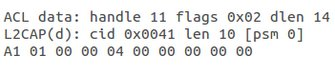
\includegraphics[scale=0.5]{hcidump.jpg}
\caption{Sample \texttt{hcidump} dump data showing capital A}
\label{fig:mypic}
\section{Executing the Attack}
To execute this attack, we used completely off-the-shelf hardware and software. The only custom software and hardware would be the incorporation of the Ubertooth device and plugin for Kismet. 
\end{figure}

\subsection{Hardware and Software}
For this attack, we wanted to test several versions of Bluetooth as well as different Operating Systems to determine how effective the attack is against different hardware and software. The following are the devices we used for the attack:

\textbf{Keyboard:} we used a basic Bluetooth keyboard that uses Bluetooth V3.0+EDR (Enhanced Data Rate (EDR), an optional speed-up of data transfer)\\
\textbf{Attack Device:} Lenovo Thinkpad z61t laptop running Ubuntu 12.04 with Bluetooth 2.0+EDR\\
\textbf{Victim Devices:} we attacked a mid-2012 Apple Macbook Air running Ubuntu 12.10 via VirtualBox with
Bluetooh 4.0 card and a desktop PC with a Bluetooth dongle, running Ubuntu 12.04 and Bluetooth 4.0.

To execute pairing, the Macbook, the Thinkpad Laptop and Tablet all use Passkey Entry authentication where a pin must be entered into the keyboard. Since the attack relies on SSP, which is largely the same across all versions of Bluetooth since it's implementation in v 2.1, the differences in Bluetooth versions across the devices should not matter. The largest variable in whether or not the attack is possible is how the OS handles the link keys and sending multiple link requests from a single address. 

\subsection{Setup}
Need a Linux laptop

\subsection{Implementation}
Note about pairing before hand
\begin{verbatim}
sudo hidd --connect <keyboard-address>
\end{verbatim}

\begin{verbatim}
sudo hcidump -x > log.out
\end{verbatim}

\begin{verbatim}
sudo ./hidclient -e8 -x
\end{verbatim}

Connect on the victim pc.
Run the python script.

\section{Results}
We successfully created a proof of concept implementation that can forward keystrokes from a Bluetooth keyboard through the attacker to a victim machine. The proof of concept currently only works in the ideal conditions.

\section{Mitigation}
We are proposing three countermeasures to prevent against Man in the Middle attacks on Bluetooth keyboards.

\begin{enumerate}
\item Stay out of discoverable mode as much as possible. This way any attacker would need special hardware to perform any kind of fancy attack and take much longer to actually find the keyboards Bluetooth address.
\item Keyboards should require a PIN to pair every time. Keyboards potentially handle much more sensitive data than a device such as a Bluetooth receiver.
\item Bluetooth manager applications should be smarter. If they notice a previously paired keyboard or device with the same name that has a different Bluetooth address that might warrant a red flag to be displayed to the user.
\end{enumerate}

\section{Future Work}
There are several obvious ways to continue the work we completed. 

\begin{enumerate}
\item Implement the entire attack. Including the denial-of-service and pairing without the users knowledge.
\item Get Ubertooth and successfully use it to choose victims without having to have prior knowledge about the victim and the keyboard.
\item Implement the entire attack in a single C/C++ application. This would make testing and debugging much easier to perform. Instead of requiring several separate tools combined together.
\item Acquire passwords!
\end{enumerate}


\section{Conclusions}
Our work shows that a Bluetooth keylogger is possible to do. We successfully forwarded packets from the keyboard to the victim with no delay. Accomplishing this task was easier said than done. We had to use several software packages in the correct order to get the behaviors we wanted. The main conclusion we came away with is that Bluetooth is needlessly complex. The API is horrible and underdeveloped. Which was not explained by any documentation we found. The documentation was useless and led us in the wrong direction 99\% of the time. If anyone could improve Bluetooth in any way we recommend making the API cleaner and standardized and improving the documentation that goes with it.

%
% The following two commands are all you need in the
% initial runs of your .tex file to
% produce the bibliography for the citations in your paper.
\bibliographystyle{abbrv}
\bibliography{refs}  % sigproc.bib is the name of the Bibliography in this case

\balancecolumns
% That's all folks!
\end{document}
